% Created 2019-07-08 Mon 22:43
% Intended LaTeX compiler: pdflatex
\documentclass[11pt]{article}
\usepackage[utf8]{inputenc}
\usepackage[T1]{fontenc}
\usepackage{graphicx}
\usepackage{grffile}
\usepackage{longtable}
\usepackage{wrapfig}
\usepackage{rotating}
\usepackage[normalem]{ulem}
\usepackage{amsmath}
\usepackage{textcomp}
\usepackage{amssymb}
\usepackage{capt-of}
\usepackage{hyperref}
\usepackage{minted}
\author{Nicolás Luarte}
\date{\today}
\title{Cynthia}
\hypersetup{
 pdfauthor={Nicolás Luarte},
 pdftitle={Cynthia},
 pdfkeywords={},
 pdfsubject={},
 pdfcreator={Emacs 25.2.2 (Org mode 9.2.3)}, 
 pdflang={English}}
\begin{document}

\maketitle
\tableofcontents

\section{Ciclos}
\label{sec:org27feb22}
\begin{center}
\begin{tabular}{lll}
Ejercicio & Protocolo & Bloque\\
\hline
Sentadilla de competencia & x6@8, 15\%, 4x7 & A\\
Sentadilla de competencia con pausa (3 ct) & x6@8, 15\%, 2x6 & A\\
Banca de competencia & x4@8, 10\%, 4x6 & A\\
Banca de competencia con pausa (5 ct) & x2@8, 15\%, 4x3 & A\\
\hline
Banca agarre cerrado & x8@8, 10\%, 3x8 & B\\
Peso muerto de competencia (sumo) & x5@8, 15\%, 3x5 & B\\
Peso muerto hasta las rodillas & x7@8, 15\%, 2x7 & B\\
Peso muerto bloques (abajo de las rodillas) & x10@8, 10\%, 2x10 & B\\
\end{tabular}
\end{center}
\section{Comentarios técnicos}
\label{sec:orgcc07480}
\subsection{04/07/2019, ciclo 1, bloque b}
\label{sec:orge128ce5}
\subsubsection{Peso muerto de competencia}
\label{sec:orgceb1371}
\begin{enumerate}
\item Buscar mantener la posición del suelo hasta abajo de las rodillas
\item Acentuar el gesto del bloqueo
\end{enumerate}
\subsection{08/07/2019, ciclo 1, bloque b}
\label{sec:org04c3ea5}
\subsubsection{Peso muerto de competencia}
\label{sec:org4800ede}
\begin{itemize}
\item Tensar la barra hasta que todo el cuerpo este en posición, y solo
ahí empezar el empuje
\item Visualiza que del suelo a las rodillas la idea es mantener la
posición y la barra bien apegada a las canillas, la suela del pie
perfectamente en el suelo
\item Luego, de las rodillas a la cadera, el movimiento es explosivo e
intenta que el bloqueo se transforme en un mero tramite
\end{itemize}
\section{Registro de progreso}
\label{sec:orga46964a}
\begin{center}
\label{tab:org0a2c746}
\begin{tabular}{lrrl}
Ejercicio & RPE & Peso & Fecha\\
\hline
Sentadilla de competencia & 8 & 90 & 03/07/2019\\
Sentadilla con pausa & 8 & 75 & 03/07/2019\\
Banca de competencia & 8 & 55 & 03/07/2019\\
Banca con pausa & 8 & 55 & 03/07/2019\\
Banca agarre cerrado & 8 & 40 & 04/07/2019\\
Peso muerto de competencia & 8 & 112.5 & 04/07/2019\\
Peso muerto hasta las rodillas & 8 & 80 & 04/07/2019\\
Peso muerto bloques & 9 & 90 & 04/07/2019\\
Sentadilla de competencia & 8 & 88 & 05/07/2019\\
Banca de competencia & 8 & 55 & 05/07/2019\\
Sentadilla con pausa & 8 & 75 & 05/07/2019\\
Banca con pausa & 8 & 55 & 05/07/2019\\
Peso muerto de competencia & 8 & 120 & 08/07/2019\\
Banca agarre cerrado & 8 & 50 & 08/07/2019\\
Peso muerto hasta las rodillas & 8 & 70 & 08/07/2019\\
Peso muerto bloques & 8 & 90 & 08/07/2019\\
 &  &  & \\
\end{tabular}
\end{center}
\begin{center}
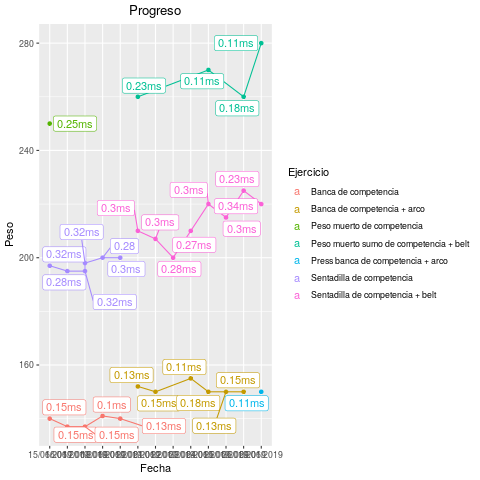
\includegraphics[width=.9\linewidth]{tmp.png}
\end{center}

\section{Tiempo de peak}
\label{sec:org187169e}
5 exposiciones
\end{document}
